\chapter{On the Effectiveness of Self-supervised Pre-training for Modeling User Behavior Sequences}

\textbf{Best paper award from AdKDD}

\textbf{Reference:}~\url{http://papers.adkdd.org/2020/papers/adkdd20-liao-effectiveness.pdf}

\textbf{Keywords:} user behavior, embeddings, CTR prediction

\section{Какую задачу решают авторы?}

История активности пользователя (какие сайты посетил, на какие объявления кликал) несет в себе полезные сигналы в том числе о комерческих интересах пользователя. \\

Использование данной информации может улучшить качество предсказания вероятности клика пользователя по объявлению (CTR prediction), так как позволяет своевременно реагировать на недавние действия пользователя.

Кроме того, в задаче CTR prediction'a очень важно постоянно обновлять модель~\cite{he2014practical}, чтобы можно было реагировать на изменения трендов в данных. \\

Большинство state-of-the-art моделей на текущий момент - это довольно массивные нейросетевые архитектуры~\cite{guo2017deepfm,zhou2018deep,wang2017deep}, которые довольно тяжело постоянно обновлять, так как это требует много времени и ресурсов, и лишь некоторые модели~\cite{zhou2018deep} используют информацию об активности пользователя. \\

В рамках статьи авторы предлагают нейросетевую архитектуру (см. Рисунок~\ref{fig:pretrainig}), состоящую из двух моделей 
\begin{itemize}
    \item \texttt{dense network} --- обрабатывает категориальные и численные признаки связанные с пользователем и объявлением
    \item \texttt{sequential network} --- обрабатывает активность пользователя
\end{itemize}

Архитектура позволяет предобучить \texttt{sequential network} в self-supervised режиме, что позволяет как быстрее переобучать модель для CTR prediction'a, так и добиваться более хороших результатов.

\section{Как решают?}

Рассмотрим детальнее что из себя представляет каждая из сетей. 

\begin{figure}[ht]
    \centering
    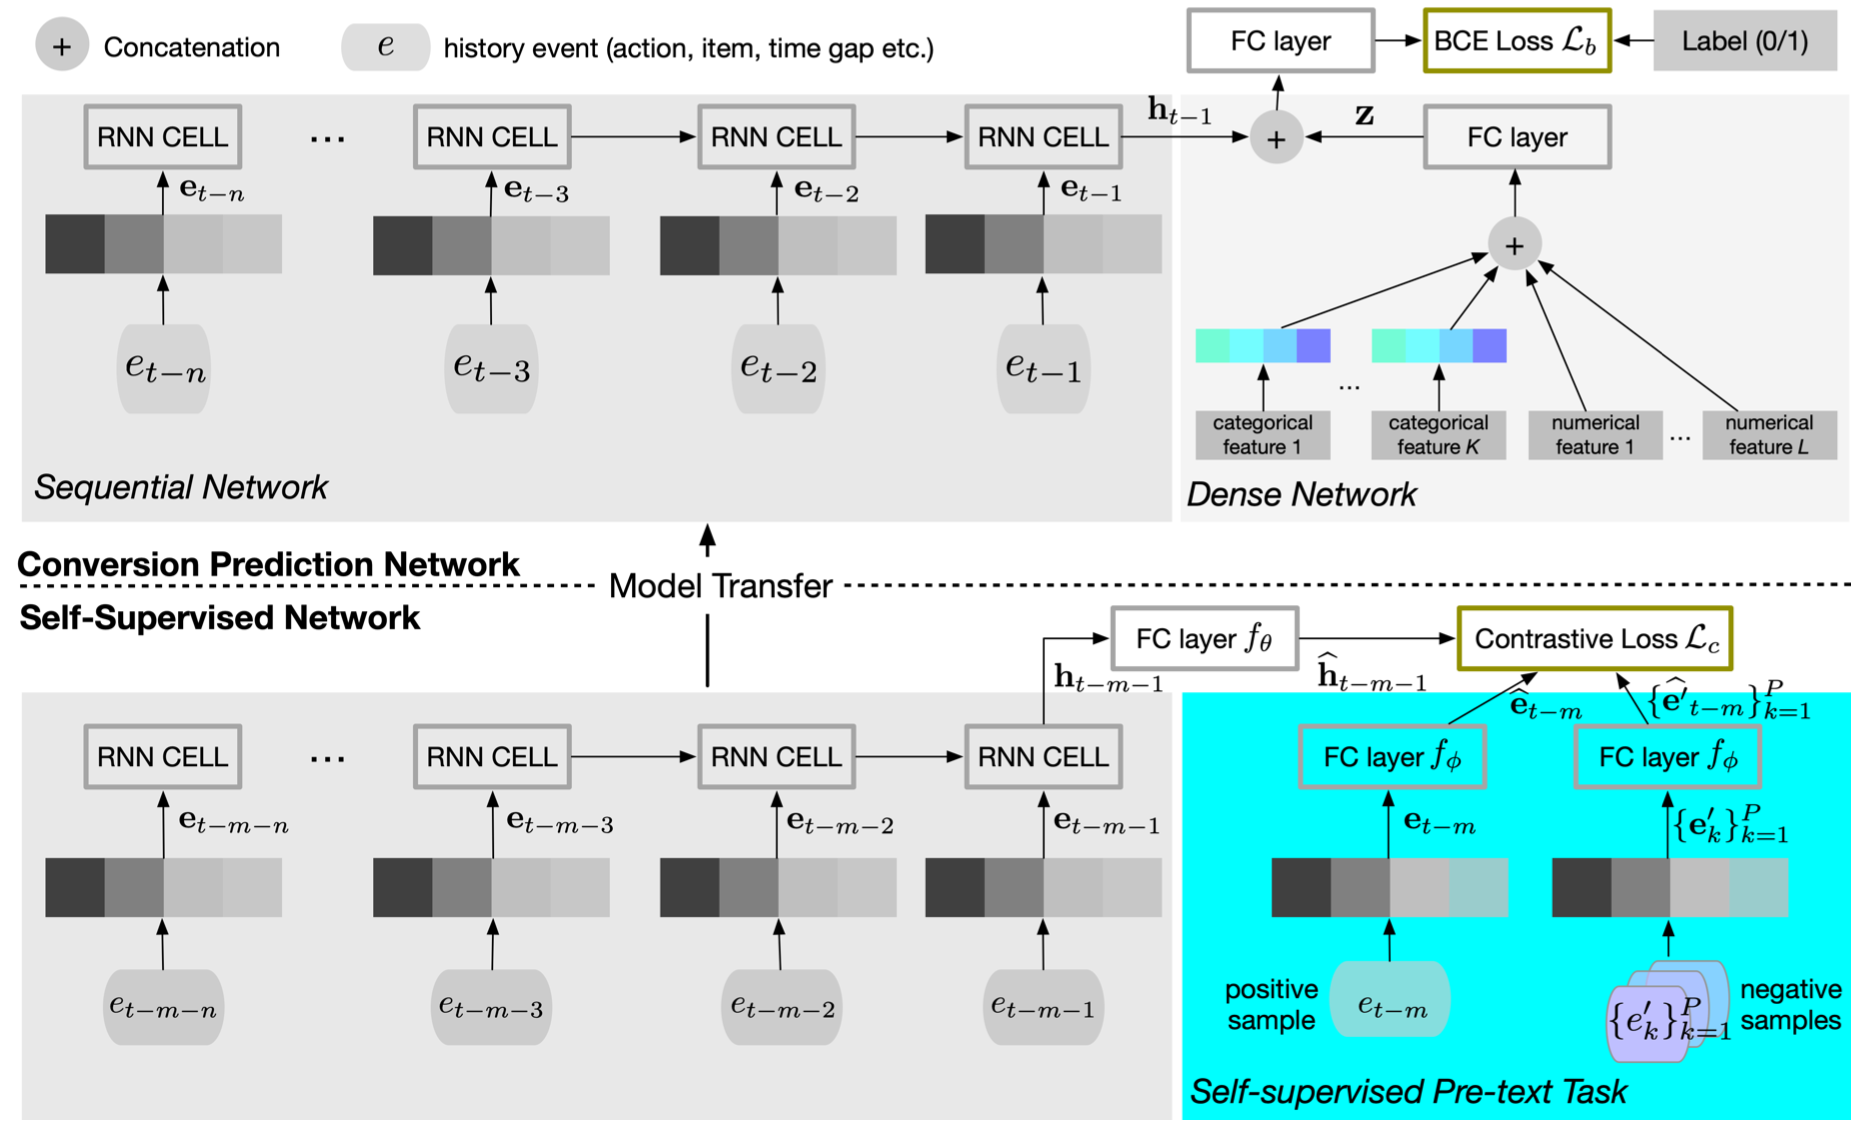
\includegraphics[width=1.0\linewidth]{images/pretraining.png}
    \caption{\small{The overview of the proposed conversion prediction and the self-supervised networks. The former consists of the sequential and the dense networks. The latter is learned by the guidance of the proposed pre-text task and it serves as the pre-trained model for the sequential network.}}
    \label{fig:pretrainig}
\end{figure}

\subsection{Dense Network}

\texttt{Dense network} имеет уже довольно привычный для задачи CTR prediction'а вид (см. Рисунок~\ref{fig:pretrainig}). \\

Для категориальных фичей обучаются эмбеддинги, которые конкатенируются с числовыми признаками и подаются на вход нескольким полносвязным слоям. \\

{\bf Remark:} в рамках работы в \texttt{dense network} подают на вход только ранжируемое объявление.

\subsection{Sequential Network}

Для того чтобы ускорить переобучение модели CTR prediction'a, авторы предлагают предобучать \texttt{sequential network} в self-supervised режиме на задаче предсказания следующего события в сессии пользователя (см. Рисунок~\ref{fig:pretrainig} нижняя часть). \\

Важно заметить, что модель обучают не напрямую предсказывать следующее событие, а обучают различать релевантные события от нерелевантных, то есть для обучения используют \texttt{contrastive loss} (Очень похоже на разницу между \texttt{CBOW} и \texttt{Skip-Gram w/ Negative Sampling} моделями для Word2Vec). \\

Использование \texttt{contrastive loss} имеет следующие преимущества в сравнении с задачей многоклассовой классификации
\begin{itemize}
    \item Обучение становится существенно быстрее, когда классов очень много. На практике, если пробовать предсказать следующий посещенный сайт, то классов могут быть миллионы. Ускорение достигается за счет того, что нет необходимости вычислять softmax для расчета итоговых вероятностей.
    \item Модель более устойчива к шуму в данных для обучения
\end{itemize}

\subsection{Итоговая модель}

Промежуточные представления полученные с помощью  \texttt{dense network} и \texttt{sequential network} конкатенируются и передаются на вход в полносвязный слой. \\

Модель обучается оптимизируя классический для задачи CTR-prediction'a лосс - \texttt{Binary Cross-Entropy loss}. \\

За счет того что \texttt{sequential network} уже была предобучена, то для обучени итоговой модели нужно как меньше данных, так и меньше времени.

\section{Преимущества подхода}

На мой взгляд, самое важное преимущество, о котором почти не написано в статье, заключается в следующем: \\

Так как модель декомпозирована на \texttt{dense network} и \texttt{sequential network}, то на этапе ранжирования нет необходимости в том, чтобы запрашивать недавнюю активность пользователя и пропускать ее через \texttt{sequential network}. 

Промежуточное представление получаемое с помощью \texttt{sequential network} можно предпосчитывать и обновлять для пользователя независимо всякий раз, когда мы получаем информацию о новых действиях пользователя, что случается гораздо реже чем ранжирование. И на этапе ранжирования достаточно для пользователя запросить уже посчитанное промежуточное представление. \\

Это существенно уменьшает время необходимое для ранжирования объявлений, так как фактически на данном этапе используется только \texttt{dense network}. \\

В статье~\cite{pi2019practice} пытались добиться такой же декомпозиции, но итоговое решение получилось очень сложным.

\section{Мое мнение}

\begin{itemize}
    \item Очень хотелось бы в качестве одного из baseline'ов увидеть решение, где в качестве \texttt{sequential network} используют просто усреднение вектора объектов из активности пользователя (вектора можно было бы обучть с помощью Word2Vec).
    \item Также было бы интересно увидеть в качестве \texttt{sequential network} и другие архитектуры, например, Bert4Rec.
    \item Жаль, что совсем не сравнивают свое решение с другими архитектурами на публичных датасетах.
\end{itemize}